\chapter {Redesign}
This chapter will present the changes that will be applied to the second further iterations, it will first present the improvements and additions that would make a better set of prototypes and then present the altered test designs.

\section{Prototype improvements and additions}
In this first iteration of the prototypes a number of things have been noted that should be improved or added to the prototypes. 
\subsection{Technical Improvements}
The implemented prototypes are all made with a focus on speed and easy to debug, this approach is useful for developing quickly. However it also means that the quality of the code produced is not as good as it could have been, this has introduced a number of problems that showed up in the tests. The following improvements can help in making the prototypes better:

\begin{itemize}

\item Make standardized controller that is static across all control schemes\\
This would be a more rigid approach to developing these prototypes this controller would then be accessible through interfaces.

\item Make the joysticks reflective of the fingers position on the screen\\
This problem is addressed in chapter \ref{DiscussionJoystick}. 


\item Refine placement of UI elements\\ 
This improvement is aimed at reducing the amount of fat-finger problems (see section \ref{MobileUsability}) that especially the buttons scheme might be prone to. While refining the placement is a simple thing it is however something that is usually done best in an iterative manner, as the users are the ones to decide where it is most effective to have them on the screen as mentioned in the user centred design section (\ref{UXUserCentred}).
\end{itemize}

\subsection{Control schemes additions}
The following items should be added to the existing prototypes, based on the user’s feedback.

\subsubsection{Common improvements for control schemes}
\begin{itemize}
\item In general all control schemes will be improved to have customizable sensitivity for both the movement and rotational speeds of the camera. This will help the users to have more personalized controls, that would suit their specific needs.

\item According to the user’s feedback, the ability to move sideways should be added to the control schemes of all further prototypes. Based on the feedback this should improve efficiency of navigation.
\end{itemize}
 \subsubsection{Joystick control scheme}\label{RedesignJoystick}
The joystick could implement adaptive placement - meaning that the joystick center is placed wherever the finger is initially placed on the screen. When the finger is taken off the screen, a new position can be initiated. (see fig. \ref{RedesignAdaptive}).

This would ensure that the users could concentrate more on the task for a better experience. This eliminates the need to focus on fixed finger placement on the screen.

\begin{figure} [H]
\centering
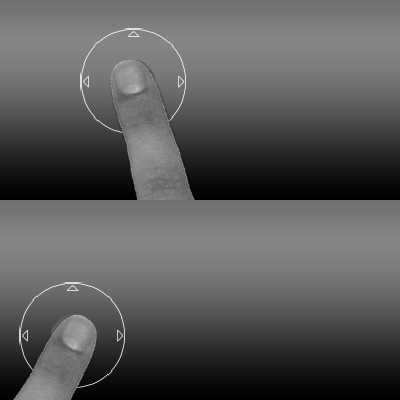
\includegraphics [scale = 0.5] {RedesignAdaptive.png}
\caption {Finger placement on joystick control}
\label {RedesignAdaptive}
\end {figure}

\subsection{Control schemes improvements}
User-centered design will be introduced in the second iteration. Users will be asked to visualize and demonstrate, how they imagine specific buttons for moving forward or backwards. This will be the foundation while redesigning the second iteration of the button graphics.


\subsection{further prototypes}\label{RedesignNewDesigns}
For the following iterations these additional prototypes will be added.
\subsubsection{Mirrored Versions}
A mirrored version of the button control scheme and the joystick control scheme.
When creating the initial prototypes not much thought was given to whether movement or rotation should be done on the right or the left side. So for the next iteration it would be interesting to switch them around, putting the movement on the right side and the rotation on the left side.
\subsubsection{Accelerometer}
Observing the users during the tests it was obvious that a lot of them mistook the gyroscope for an accelerometer, tilting the device instead of rotating around with the device. From this an assumption can be made that the accelerometer is more familiar to the target group than the gyroscope. Therefore, making a prototype that employs the accelerometer for navigation would be an obvious next step.
The users would use the device as a steering wheel as when driving a car. As shown in figure \ref{RedesignAccelerometer}
\begin{figure} [H]
\centering
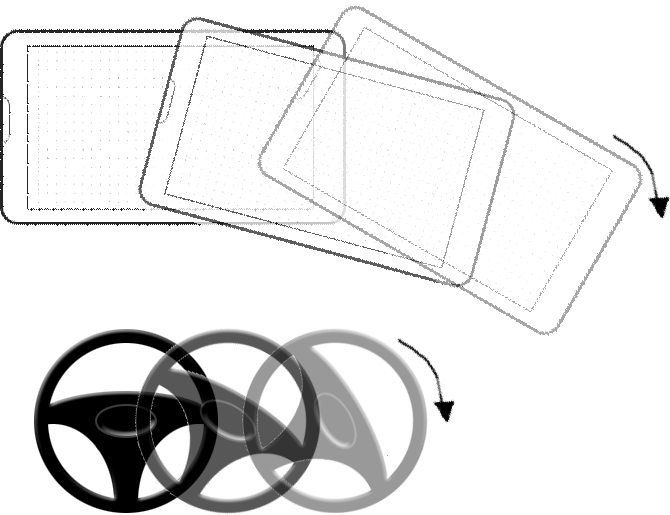
\includegraphics [scale = 0.5] {RedesignAccelerometer.png}
\caption {Example of real-world familiarity regarding the accelerometer}
\label {RedesignAccelerometer}
\end {figure}

\subsubsection{Joystick and gyroscope fusion}\label{RedesignJoyGyro}
While observing the test participants interact with the joystick control scheme, it seemed the movement of the joystick was the most prefered part of it. However the test participants did not enjoy the camera rotation for this layout. The most prefered camera rotation controls seemed to be the gyroscope.
Combining the movement from the joystick with the camera rotation from the gyroscope could shape a more enjoyable control scheme. In addition this would also allow the user to control everything with a single hand.

\section{Redesigning the test}
This section will describe the testing for the second iteration and further iterations.
Further testing of the navigation will be focused on the rotational functionality of each control scheme for which the initial test-level was designed for. 

\subsection{Testing Efficiency}
For additional efficiency testing it would be crucial to compare the control schemes after the test participants get a chance to play with the controls and become familiar with them.
That way the focus would be on the actual efficiency of the controls and not on how fast they learn them.
Another important thing would be to switch the focus of the test from navigating through an obstacle course to focus on rotational movement. The obstacle course encouraged the test participants to put their effort into the movement more so than looking around. The hypothesis here is that while simple movement and navigation favours the button controls, while tasks involving camera rotation might favour one of the less traditional control schemes.

\subsection{UX Testing} 
For future iterations the user experience will need to be measured.
Instead of just looking at usability as it has been done in the first iteration, it would be interesting to also look deeper into the user experience and test to which extend the efficiency influence the user experience.
This can be achieved by repeating the test from the first iteration, while changing the premises to be non-competitive and asking the test participants to also describe their experience.
The main focus would be on observing the user's emotional reactions, instead of the completion times.

